% !TeX root = RJwrapper.tex
\title{Navigating the R Package Universe}
\author{by Spencer Graves, John C. Nash, Julia Silge}

\maketitle

\abstract{%
An abstract of less than 150 words.
}

\subsection{Introduction}\label{introduction}

As of our writing, there are more than 12,000 packages on CRAN. R users
must approach this abundance of packages with effective strategies to
find what they need and choose which packages to invest time in learning
how to use. At useR!2017 in Brussels, we organized a contributed session
centered on this issue, with three themes in our discussion. The three
themes we focused on are \textbf{search}, \textbf{guidance}, and
\textbf{unification}. Here, we summarize these important themes, the
discussion in our community both at useR!2017 and in the intervening
months, and where we can go from here.

Users need options to search R packages, perhaps the content of
DESCRIPTION files, documentation files, or other components of R
packages. One author (Graves) has worked on the issue of searching for R
functions from within R itself in the sos package \citep{sos}, and other
options have been built such as RDocumentation.org
\citep{rdocumentation}.

Guidance about what package to use for any given task is available from
multiple resources for users. R users can turn to long-established
resources like CRAN Task Views (reference?), or newer options under
current development such as the packagemetrics package
\citep{packagemetrics} or the CRANsearcher RStudio addin
\citep{cransearcher}. One author (Silge) organized a survey before useR
about how R users learn about R packages that informed our discussion
and is summarized here.

By unification, we largely mean meta-packages or wrappers, packages that
call other, related packages for a common set of tasks. With a unified
wrapper package, a user only has to learn one API but then can use many
different implementations for a certain task. One author (Nash) has been
particularly involved in numerical optimization techniques and presented
possibilities there and beyond. More generally, as revealed during
breakout discussions at useR!2017 and beyond, there are opportunities to
merge either packages or their functionality. Such ideas require human
cooperation and some give and take in a realm where egos can take
precedence over the efficiency of the R ecosystem.

After our main presentation at useR!2017, we broke out into three
smaller sessions focused on these three themes. We are encouraged by the
engaged attendance and vigorous participation from the community we
experienced, and hope to use our community's enthusiasm and ideas to
move forward with steps that will improve parts of the R ecosystem.

You can include references in parentheses \citep{R}, or cite a reference
such as \citet{R} in the text.

\subsection{Search}\label{search}

\subsection{Guidance}\label{guidance}

In preparation for this session, one author (Silge) ran a brief online
survey in the spring of 2017 to ask R users how they currently discover
and learn about R packages. The results of this survey are available in
an R package \citep{packagesurvey} on GitHub. There were 1039
respondents to this survey, which had a single multiple select question
on it, ``How do you currently discover and learn about R packages?''

\begin{Schunk}
\begin{table}

\caption{\label{tab:unnamed-chunk-2}Percentage of respondents who chose each answer on survey}
\centering
\begin{tabular}[t]{ll}
\toprule
How do you currently discover and learn about R packages? & \% of respondents\\
\midrule
Social media such as blogs, R-bloggers, Twitter, Slack, or GitHub contacts & 79.8\%\\
General search websites such as Google and Yahoo & 57.0\%\\
Your personal network, such as colleagues and professors & 41.6\%\\
Books, textbooks, or journal articles (JSS, JOSS, R-Journal) & 31.9\%\\
Conferences, meet-ups, or seminars & 24.1\%\\
\addlinespace
CRAN Task Views & 21.8\%\\
Email lists such as r-help, r-packages, or r-pkg-devel & 15.3\%\\
R-specific search websites such as METACRAN or Rdocumentation & 11.1\%\\
Other & 4.2\%\\
R packages built for search such as the sos package & 2.2\%\\
\bottomrule
\end{tabular}
\end{table}

\end{Schunk}

Responses to this survey were fielded from R email help lists, local R
meetup groups, social media such as Twitter, and affinity groups such as
R-Ladies. Figure 1 shows when users responded to the survey. The
respondents to this survey overwhelmingly look to social media including
blogs and Twitter to learn about R packages, and also make use of
general search sites and their personal network.

There were helpful, insightful answers from people contributing to the
``other'' option. R users use
\href{https://stackoverflow.com/questions/tagged/r}{Stack Overflow} to
learn about R packages, as well as options like
\href{http://dirk.eddelbuettel.com/cranberries/}{CRANberries} and
\href{http://www.crantastic.org/}{crantastic}, both of which have RSS
feeds that users follow. Other users mentioned learning by reading code
on GitHub, and other search websites including
\href{http://rpackages.io/}{rpackages.io}.

\begin{Schunk}
\begin{figure}
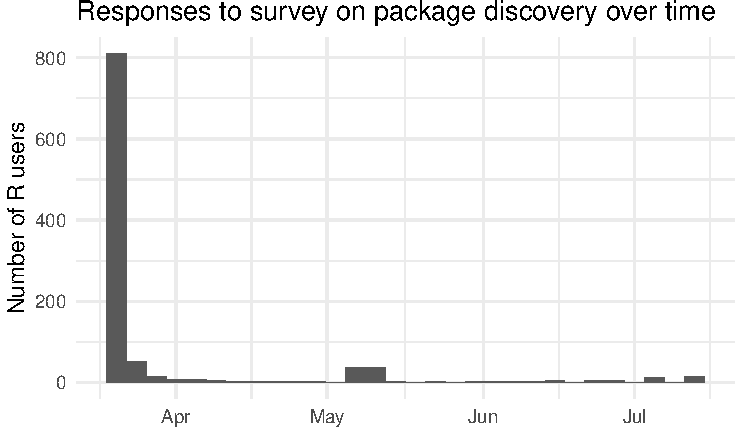
\includegraphics{navigating_files/figure-latex/survey_time-1} \caption[Responses to survey on package discovery during the spring of 2017]{Responses to survey on package discovery during the spring of 2017}\label{fig:survey_time}
\end{figure}
\end{Schunk}

At useR!2017, after the large contributed session, we broke out into
three smaller sessions for discussion and brainstorming. In the breakout
session focused on guidance for package choice and package evaluation,
we had about 40 participants in our discussion. It was a fruitful
discussion and several important themes emerged.

\subsubsection{Value of personal impact}\label{value-of-personal-impact}

Participants in this session emphasized how impactful personal
relationships can be in how packages are shared and evaluated. Some
participants discussed how building local networks of R users may be
more important in this effort than top-down, technological solutions.
Our survey does show that personal recommendations have been important
for many individuals in evaluating R packages. This is yet another area
where local user groups can continue to have important impact. Some ways
to share this experience more broadly would be online video series or
live data analysis, such as those by
\href{https://www.facebook.com/seanjtaylor/videos/10103088186201897/?pnref=story}{Sean
Taylor} and
\href{https://twitter.com/rdpeng/status/872090694390861824}{Roger Peng}.

\subsubsection{CRAN Task Views}\label{cran-task-views}

Some participants wondered whether the idea of a
\href{https://cran.r-project.org/web/views/}{CRAN Task View} is outdated
in the current climate with so many packages, and whether it is even
possible for one person to maintain one effectively. Others responded
that CTVs are all about curation, which is still important, perhaps even
more important now. We had at least one CTV maintainer present in our
breakout session, and several things were presented as important in
order for CTV maintainers to do their jobs:

\begin{itemize}
\tightlist
\item
  Package maintainers should update their \texttt{NEWS} files.
\item
  Package maintainers need to write good documentation.
\end{itemize}

These are helpful for \emph{all} R users, of course, but also for
maintainers of CRAN Task Views. The pkgdown \citep{pkgdown} package was
mentioned as a great way to make documentation visible.

\subsubsection{\texorpdfstring{CRAN and
\emph{you}}{CRAN and you}}\label{cran-and-you}

Participants had several ideas about how things are done on CRAN now and
adjustments that might be made in the interest of discovering and
evaluating packages. One idea that came up several times was the
possibility of keywords or tagging for packages. Since useR!2017, the
authors have learned that there is support for some tagging architecture
for packages on CRAN in the
\href{https://cran.r-project.org/doc/manuals/r-release/R-exts.html\#The-DESCRIPTION-file}{DESCRIPTION
file using ACM, JEL, or MSC classifications}. For an example of this in
action, check out the lfe \citep{lfe} package. These are fairly unwieldy
lists currently and something like an RStudio addin could be used to
navigate them, if they were widely used.

Another desire participants voiced was for more information directly on
CRAN, such as the number of downloads for packages. Participants also
suggested that vignettes for context-specific tasks like the
\href{https://www.bioconductor.org/help/workflows/}{Bioconductor
Workflows} would be helpful for package discovery and evaluation, either
associated with CRAN or perhaps the \emph{R Journal}. Finally, there was
some discussion about whether the very minimal gate-keeping on CRAN was
good or bad for the community, although the general feeling was that
efforts to keep packages off CRAN would not be positive.

\subsubsection{More data, more problems}\label{more-data-more-problems}

Some of the package developers at the session wondered why, when R is a
data-centric language, developers have such primitive analytics about
their users. Issues of user privacy are central here, but there might be
opt-in options that could help both package developers and users make
better decisions. The idea of a recommender system for R packages was
brought up multiple times, perhaps a Tinder for R packages like
\href{https://simplystatistics.org/2016/10/03/papr/}{papr, the Tinder
for academic preprints}. Both the users and developers present thought
that data on package use (instead of package downloads alone) would be
helpful in evaluating how important or helpful R packages are.
Participants also discussed the possibility of a linter for analysis
scripts, similar in concept to linters for code (such as \citet{lintr}),
that would suggest packages and good practice. Such a linter would
necessarily be opinionated, but almost all of the efforts to suggest and
evaluate R packages are at some level.

\subsection{Unification}\label{unification}

\subsection{Summary}\label{summary}

Our work on these topics leads us to call for increased respect and
value for the work done by local meetup group organizers and individuals
who contribute to spreading R knowledge, both online and in their
communities. Our survey and discussions show how impactful these
community networks are; investing in community building is not something
we need do only because of idealism, but because it is effective.

We can also see the importance of continued commitment to growing the
skills of package developers across the R ecosystem. Adopting best
practices, including writing good documentation, makes this entire
challenge better for everyone, from the CRAN Task View maintainer to the
new R user.

JOHN AND SPENCER: For full details of \emph{The R Journal} style and
information on how to prepare your article for submission, see the
\href{https://journal.r-project.org/share/author-guide.pdf}{Instructions
for Authors}. \bibliography{RJreferences}

\address{%
Spencer Graves\\
EffectiveDefense.org\\
line 1\\ line 2\\
}
\href{mailto:spencer.graves@effectivedefense.org}{\nolinkurl{spencer.graves@effectivedefense.org}}

\address{%
John C. Nash\\
University of Ottawa\\
line 1\\ line 2\\
}
\href{mailto:nashjc@uottawa.ca}{\nolinkurl{nashjc@uottawa.ca}}

\address{%
Julia Silge\\
Stack Overflow\\
110 William Street, Floor 28\\ New York City, NY 10038\\
}
\href{mailto:julia.silge@gmail.com}{\nolinkurl{julia.silge@gmail.com}}

